%! suppress = MissingLabel
%! suppress = LineBreak
\section{Разработка системы генерации оружия}

В этой главе описывается разработка системы генерации оружия. Исходный код доступен в репозитории\cite{s7}. WebGL демо доступно здесь\cite{s9}. У проекта есть документация на английском\cite{s13}.

\textbf{Замечание.} Система предназначена для работы внутри игрового движка Unity, поэтому WebGL демо не может показать весь её функционал. В WebGL демо не доступно изменение параметров оружия, сохранение и загрузка параметров и генома, выбор понравившегося оружия для создания следующего поколения. Для тестирования этих функций системы потребуется выполнить следующие шаги:

\begin{enumerate}
    \item Установите Unity версии 2022.3 или новее.
    \item Клонируйте репозиторий с проектом\cite{s7}.
    \item Откройте директорию с репозиторием как проект Unity. Все зависимости будут установлены автоматически.
\end{enumerate}

\subsection{Цвет и траектория снарядов}

В этом параграфе описан упрощенный алгоритм управления снарядами нейронной сетью, который может отличаться от того, что представлено в исходном коде. Этот алгоритм выполняется каждый кадр игры.

\lstset{
    emph={InverseTransformPoint, TransformDirection, AddForce, ResetState, Activate, SqrMagnitude, Sqrt, Lerp, Abs, HSVToRGB},
    emphstyle=\color{mauve},
    emph={[2]Mathf, math, Vector2, Color, NeatGenomeParams},
    emphstyle={[2]\color{dkgreen}}
}

\pagebreak

\begin{lstlisting}[name=Projectile, caption={Projectile. Part 1}]
Box.ResetState(); 

Vector2 RelativePos = transform.localPosition;
float DistanceFromOrigin = RelativePos.magnitude;
float maxDistance = NNControlDistance * math.SQRT2;

_inputArr[0] = Mathf.Lerp(-1f, 1f, Mathf.Abs(RelativePos.x) / NNControlDistance);
_inputArr[1] = Mathf.Lerp(-1f, 1f, Mathf.Abs(RelativePos.y) / NNControlDistance);
_inputArr[2] = Mathf.Lerp(-1f, 1f, DistanceFromOrigin / maxDistance);
            
Box.Activate();
\end{lstlisting}

Рассмотрим подробнее этот фрагмент кода. \lstinline{_inputArr[]} -- это массив, через который нейронная сеть получает данные. Все значения, принимаемые нейронной сетью должны лежать в отрезке $[-1,1]$. Для нормализации входных данных используется встроенный в Unity метод для линейной интерполяции \lstinline{Lerp()}, а также параметр \lstinline{NNControlDistance}, подбираемый пользователем.

Чтобы у пользователя была возможность менять направление полета снарядов относительно оси у на противоположное, их паттерн должен быть симметричен относительно этой оси. Также для более приятного визуального эффекта было решено сделать паттерн симметричным и относительно оси х. Для этого в сеть подаётся модуль первых двух параметров, отвечающих за координаты.

Если обобщить, то в коде выше берутся актуальные для данного кадра позиция снаряда \lstinline{RelativePos}, его расстояние от источника \lstinline{DistanceFromOrigin} и подаются на вход в нейронную сеть после нормализации. Затем происходит активация сети \lstinline{Box.Activate()}.



\pagebreak

\begin{lstlisting}[name=Projectile, caption={Projectile. Part 2}]
float x = Mathf.Lerp(-1f, 1f, (float)_outputArr[0]) * SignX;
float y = Mathf.Lerp(-1f, 1f, (float)_outputArr[1]) * SignY;    
Vector2 forceDir = OriginTransform.TransformDirection(x, y, 0f).normalized;
    
float hue, maxSpeed, force;
hue = Mathf.Lerp(HueRange.x, HueRange.y, (float)_outputArr[2]);
maxSpeed = Mathf.Lerp(SpeedRange.x, SpeedRange.y, (float)_outputArr[3]);
force = Mathf.Lerp(ForceRange.x, ForceRange.y, (float)_outputArr[4]);

SpriteRenderer.color = Color.HSVToRGB(hue, Saturation, Brightness);
Rigidbody.AddForce(forceDir * force);

float speed = Rigidbody.velocity.magnitude;
if (speed > maxSpeed)
    Rigidbody.velocity = Rigidbody.velocity.normalized * maxSpeed;

transform.up = Rigidbody.velocity;
\end{lstlisting}

После активации сети можно считывать выходные данные через массив \lstinline{_outputArr[]}. Сеть выдает все значения в отрезке $[0,1]$. Данные с первых двух выводов \lstinline{_outputArr[0]} и \lstinline{_outputArr[1]}, отвечающих за $x$ и $y$ компоненты вектора, сначала преобразуются в отрезки $[-1,1]$. Затем на их основе строится нормированный вектор \lstinline{forceDir}, который потом прилагается к снаряду посредством метода \lstinline{AddForce}.

Так было сделано для плавности и реалистичности полета снарядов, если бы нейронная сеть меняла их скорость напрямую, они бы двигались дёрганно и слишком резко. Чтобы под действием силы скорость снаряда не росла до бесконечности, она ограничена параметром \lstinline{maxSpeed}.

Изначально планировалось использовать цветовую модель RGB, но возникли проблемы с контролем цветов, которые может выдавать сеть. Например, если у игры темный фон, то снаряды должны быть ярких оттенков, чтобы не сливаться с ним. У пользователя должна быть возможность задать желаемое пространство цветов, внутри которого будут заключены значения нейронной сети. RGB представляет цвета в виде точек в трехмерном пространстве, поэтому выделить такое пространство было бы затруднительно.

Эту проблему решает цветовая модель HSV (Hue, Saturation, Value — тон, насыщенность, значение), в которой цвет представляется более интуитивно понятным образом. Компонента {\small \textbf{hue}} задается в виде отрезка, минимальное и максимальное значение которого выбирается пользователем. {\small \textbf{Saturation}} и {\small \textbf{Value}} задаются как константы и тоже могут быть изменены пользователем.



\subsection{Параметры оружия}
Был добавлен 31 параметр, чтобы предоставить пользователю возможность точной настройки оружия.

\vspace{5mm}

\textbf{Параметры стрельбы.} Эти параметры регулируют скорострельность и начальную фазу полёта снарядов:
\begin{enumerate}
    \item {\small \textbf{FireRate}} -- Время в секундах между каждой очередью или выстрелом.
    \item {\small \textbf{ProjectilesInOneShot}} -- Количество снарядов в очереди или выстреле.
    \item {\small \textbf{WeaponMode}} -- Определяет режим стрельбы. Их два:
    \begin{enumerate}[label=\textbullet]
        \item {\small \textbf{MultiShot}} -- Одиночный выстрел, состоящий из множества снарядов. Снаряды вылетают полукругом, который определяется параметром {\small \textbf{Angle}}.
        \item {\small \textbf{Burst}} -- Очередь, при которой снаряды вылетают по одному.
    \end{enumerate}
    \item {\small \textbf{BurstMode}} -- Определяет подвид стрельбы очередью. Их шесть:
    \begin{enumerate}[label=\textbullet]
        \item {\small \textbf{Clockwise}} -- Снаряды вылетают полукругом. Первый с максимальным углом, последний с минимальным. {\small \textbf{SignX}} у первой половины положительный, у второй -- отрицательный.
        \item {\small \textbf{CounterClockwise}} -- Снаряды вылетают полукругом. Первый с минимальным углом, последний с максимальным. {\small \textbf{SignX}} у первой половины отрицательный, у второй -- положительный.
        \item {\small \textbf{Alternate}} -- Начальные траектории снарядов чередуются от большего угла к меньшему. {\small \textbf{SignX}} чередует знак.
        \item {\small \textbf{Straight}} -- Снаряды летят прямо. {\small \textbf{SignX}} чередуется знак.
        \item {\small \textbf{MaxMinAngle}} -- Одна половина снарядов летит с максимальным углом, другая -- с минимальным.
        \item {\small \textbf{Random}} -- Угол и знак {\small \textbf{SignX}} выбираются случайно.
    \end{enumerate}
    \item {\small \textbf{BurstRate}} -- Время в секундах между снарядами при стрельбе очередью.
\end{enumerate}

\vspace{5mm}

\textbf{Параметры систем координат.} Системы координат являются родителями снарядов в иерархии сцены, поэтому при их движении движутся и снаряды. Регулируя эти параметры, можно создавать более сложное оружие:
\begin{enumerate}
    \setcounter{enumi}{5}
    \item {\small \textbf{RotationSpeed}} -- Вращение систем координат в градусах в секунду при нажатии кнопки запуска. Если значение отрицательное, вращение будет в противоположном направлении.
    \item {\small \textbf{MoveSpeed}} -- Скорость систем координат при нажатии кнопки запуска.
\end{enumerate}

\vspace{5mm}

\textbf{Параметры снарядов.} Эти параметры отвечают за поведение и внешний вид снарядов:
\begin{enumerate}
    \setcounter{enumi}{7}
    \item {\small \textbf{NetworkControlMode}} -- Определяет, как нейронная сеть управляет снарядом. Есть два режима:
    \begin{enumerate}[label=\textbullet]
        \item {\small \textbf{ForceSum}} -- Сеть выдает вектор силы, который затем суммируется с вектором силы, уже действующим на снаряд.
        \item {\small \textbf{VelocitySum}} -- Сеть выдает вектор скорости, который затем суммируется с вектором скорости, которым уже обладает снаряд.
    \end{enumerate}
    \item {\small \textbf{ReadMode}} -- Определяет, каким образом из выводов сети $(x, y)$ формируется вектор $\overrightarrow{dir}$, определяющий направление скорости или силы. Есть два режима:
    \begin{enumerate}[label=\textbullet]
        \item {\small \textbf{Default}}: \[ \overrightarrow{dir}=x\hat{x}+y\hat{y}, \]
        где $\hat{x}, \hat{y}$ -- орты локальной системы координат снаряда с началом в точке выстрела.

        \item {\small \textbf{Rotator}}: \[ \overrightarrow{dir}=x\hat{q}+y\hat{r}, \]
        где $\hat{r}$ -- орт радиус-вектора снаряда, и $\hat{q} \perp \hat{r}$.

    \end{enumerate}
    \item {\small \textbf{Size}} -- Размер снаряда. Для рендеринга снарядов используется текстура круга. Изменяя этот параметр, можно получать снаряды овальной формы.
    \item {\small \textbf{HasLifespan}} -- Имеется ли у снаряда срок жизни, по истечении которого он уничтожается.
    \item {\small \textbf{Lifespan}} -- Срок жизни снаряда в секундах.
    \item {\small \textbf{HasTrail}} -- Оставляет ли снаряд за собой след.
    \item {\small \textbf{HueRange}} -- Диапазон возможных значений для цветовой компоненты hue. Точное значение зависит от вывода нейронной сети.
    \item {\small \textbf{Saturation}} -- Цветовая компонента Saturation.
    \item {\small \textbf{Brightness}} -- Цветовая компонента Value.
\end{enumerate}

\vspace{5mm}

\textbf{Параметры паттерна.} Эти параметры определяют настройки, связанные вводами и выводами нейронной сети:
\begin{enumerate}
    \setcounter{enumi}{16}
    \item {\small \textbf{SpeedRange}} -- Диапазон возможных значений для максимальной скорости снаряда. Точное значение зависит от вывода нейронной сети.
    \item {\small \textbf{ForceRange}} -- Диапазон возможных значений силы, приложенной к снаряду. Точное значение зависит от вывода нейронной сети.
    \item {\small \textbf{NNControlDistance}} -- Определяет область, в которой снаряды управляются нейронной сетью.
    \item {\small \textbf{SignX}} -- Множитель вывода \textbf{x}. Если он равен нулю, вывод будет проигнорирован.
    \item {\small \textbf{SignY}} -- Множитель вывода \textbf{y}. Если он равен нулю, вывод будет проигнорирован.
    \item {\small \textbf{ForwardForce}} -- Прилагать ли к снаряду силу, направленную вперед. Эта сила равна выводу {\small \textbf{force}} нейронной сети.
\end{enumerate}

\vspace{5mm}

\textbf{Параметры начальной фазы:}
\begin{enumerate}
    \setcounter{enumi}{22}
    \item {\small \textbf{InitialFlightRadius}} -- Определяет область, в которой снаряды находятся в состоянии начальной фазы. В этом состоянии снаряды не управляются нейронной сетью, вместо этого они движутся с постоянной начальной скоростью.
    \item {\small \textbf{InitialSpeed}} -- Длина вектора начальной скорости.
    \item {\small \textbf{Angle}} -- Максимальный угол в градусах между начальной скоростью снаряда и вертикальной осью игрового объекта оружия.
\end{enumerate}

\vspace{5mm}

\textbf{Параметры отражения:}
\begin{enumerate}
    \setcounter{enumi}{25}
    \item {\small \textbf{FlipXOnReflect}} -- Изменять ли значение {\small \textbf{SignX}} на противоположное после отражения.
    \item {\small \textbf{FlipYOnReflect}} -- Изменять ли значение {\small \textbf{SignY}} на противоположное после отражения.
    \item {\small \textbf{Mode}} -- Определяет границы, от которых снаряд отражается. Есть три режима:
    \begin{enumerate}[label=\textbullet]
        \item {\small \textbf{CircleReflection}} -- Границей является окружность.
        \item {\small \textbf{RectangleReflection}} -- Границей является прямоугольник.
        \item {\small \textbf{Polar}} -- Границей является угол.
    \end{enumerate}
    \item {\small \textbf{ReflectiveCircleRadius}} -- Радиус границы-окружности.
    \item {\small \textbf{RectDimensions}} -- Размеры границы-прямоугольника.
    \item {\small \textbf{MaxPolarAngleDeg}} -- Максимально возможный полярный угол в градусах.
\end{enumerate}



\pagebreak


\subsection{Пользовательский интерфейс}

Для создания кастомных окон инспектора использовалась система\\ IMGUI\cite{s10}, которая предназначена для расширения функциональности Unity и разработки инструментов для разработчиков.

\begin{figure}[ht]
    \begin{center}
        \scalebox{0.6}{
            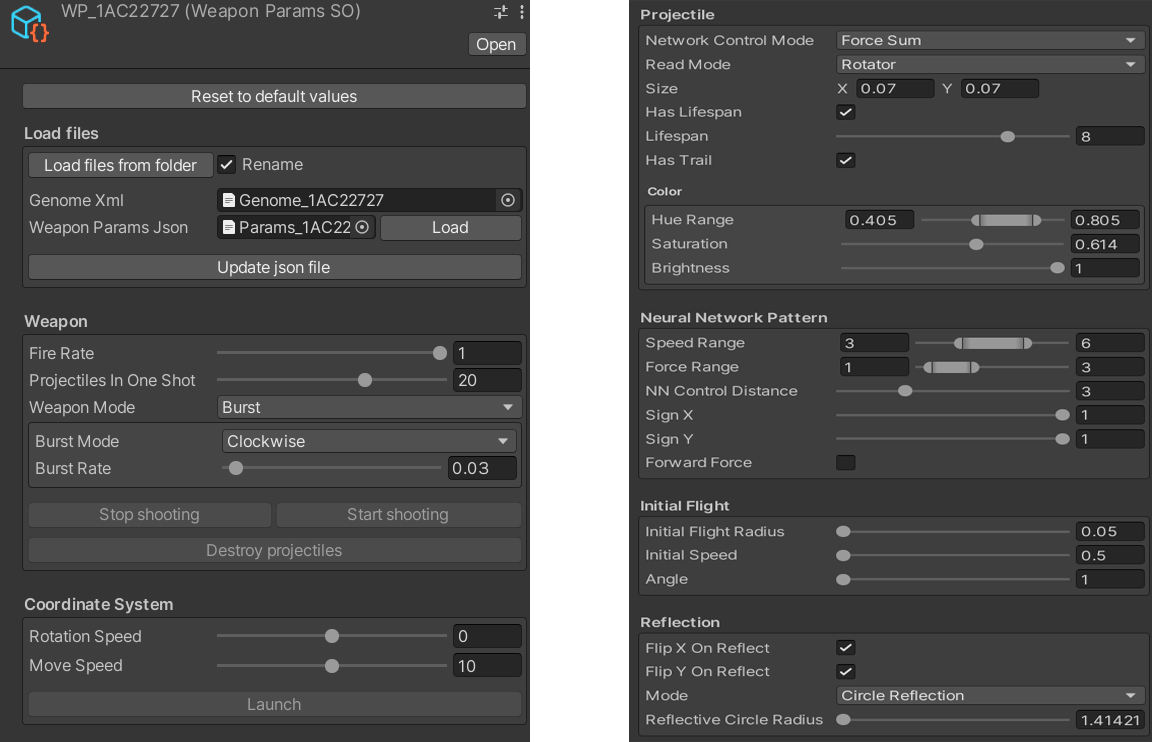
\includegraphics{images/WP3}
        }

        \caption{
            \label{Inspector}
            Кастомный инспектор параметров оружия.}
    \end {center}
\end {figure}

Функции и особенности инспектора параметров оружия (Рисунок~\ref{Inspector}):
\begin{enumerate}[label=\textbullet]
    \item Кнопка {\small \textbf{Reset to default values}}, возвращающая параметры к начальным значениям.
    \item Раздел {\small \textbf{Load files}} для загрузки генома и параметров оружия с файлов.
    \item Кнопка {\small \textbf{Update json file}}, позволяющая перезаписать значения json файла значениями, которые выбраны в инспекторе в данный момент.
    \item Кнопки {\small \textbf{Stop shooting}} и {\small \textbf{Start shooting}}, позволяющие останавливать и начинать стрельбу. 
    \item Кнопка {\small \textbf{Destroy projectiles}}, уничтожающая снаряды.
    \item Кнопка {\small \textbf{Launch}}, запускающая вращение и движение систем координат, в которых находятся снаряды.
    \item Двойные слайдеры, позволяющие задавать два значения: минимальное и максимальное.
    \item Интерфейс подстраивается под выбранные значения. К примеру, если в параметре {\small \textbf{Weapon Mode}} будет выбран режим {\small \textbf{Burst}}, появятся поля {\small \textbf{Burst Mode}} и {\small \textbf{Burst Rate}}.
    \item Есть поддержка редактирования нескольких объектов.
    \item Есть поддержка истории редактирования. То есть Undo/Redo.
\end{enumerate}


\vspace{5mm}

\begin{figure}[ht]
    \begin{center}
        \scalebox{0.6}{
            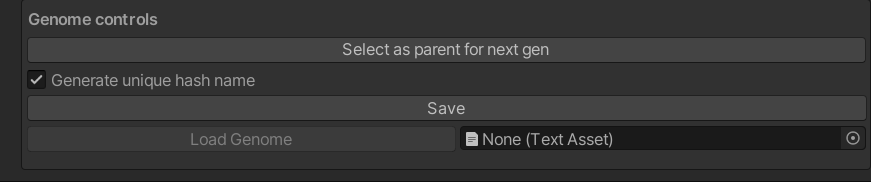
\includegraphics{images/savingWeapons}
        }

        \caption{
            \label{SavingWeapon}
            Кастомный инспектор оружия.}
    \end {center}
\end {figure}

Функции и особенности инспектора оружия (Рисунок~\ref{SavingWeapon}):
\begin{enumerate}[label=\textbullet]
    \item Кнопка {\small \textbf{Select as parent for next gen}}, позволяющая пользователю выбирать понравившиеся геномы.
    \item Кнопка {\small \textbf{Save}} для сохранения генома и параметров оружия.
    \item Флажок {\small \textbf{Generate unique hash name}}. Если отмечен, то при сохранении названия файлов генерируются автоматически.
    \item Есть поддержка редактирования нескольких объектов.
\end{enumerate}


\subsection{Система эволюции оружия}

\textbf{Выбор библиотеки.} Для эволюции нейронных сетей была выбрана библиотека SharpNEAT\cite{s8} версии 2.4.4, реализующая алгоритм NEAT на языке C\#. Выбор этой библиотеки и её версии обусловлен в первую очередь совместимостью с игровым движком Unity.

Существует SharpNEAT версии 4.0.0, в которой значительно улучшена производительность и удобство программного интерфейса, но целевая платформа этой версии -- .NET Core, несовместимая с Unity. По этой причине выбор остановился на более ранней версии 2.4.4.

Для использования библиотеки в Unity необходимо создать её DLL в какой-либо среде разработки и поместить эту DLL в специальную папку \flqq Plugins\frqq. Плагины в Unity могут быть на трех языках: C, C++, C\#. Плагины на C\# доступны в бесплатной версии Unity, а вот для использования плагинов на других двух языках придется покупать профессиональную версию.




\textbf{Параметры алгоритма NEAT.} Обычно NEAT используют для эволюции огромного количества нейронных сетей на протяжении множества поколений с помощью функции приспособленности, заданной математически. В нашем случае функцией приспособленности является человек -- игрок или разработчик игры, поскольку задача оценки эстетичности и полезности паттернов не является строго формализируемой. По этой причине оцениваемая популяция и количество поколений не должны быть большими.

Приведенные ниже значения параметров были получены опытным путем, остальные параметры сохранили значение по умолчанию. Параметры подбирались таким образом, чтобы интересные паттерны в среднем выводились за 10-15 поколений.

\begin{lstlisting}[caption={Параметры алгоритма эволюции}]
PopulationSize = 6;
CloneOffspringCount = 2;
SexualOffspringCount = 4;
NeatGenomeParams.FeedforwardOnly = true,
NeatGenomeParams.InitialInterconnectionsProportion = 0.8;
NeatGenomeParams.DisjointExcessGenesRecombinedProbability = 0.3;
NeatGenomeParams.ConnectionWeightMutationProbability = 0.8;
NeatGenomeParams.AddNodeMutationProbability = 0.6;
NeatGenomeParams.AddConnectionMutationProbability = 0.6;
NeatGenomeParams.NodeAuxStateMutationProbability = 0.1;
NeatGenomeParams.DeleteConnectionMutationProbability = 0.1
\end{lstlisting}



\textbf{Создание нового поколения.} Для создания нового поколения оружия необходимо выбрать родителей, на основе которых оно построится. Пользователь может выбрать любое их количество:

\begin{enumerate}[label=\textbullet]
    \item Если пользователь не выбрал ни одного генома, программа случайно выберет два.
    \item Если пользователь выбрал один геном, то этот геном будет скрещен с не выбранными.
    \item Если пользователь выбрал два или более геномов, то выбранные геномы будут скрещены между собой.
\end{enumerate}

\begin{figure}[ht]
    \begin{center}
        \scalebox{0.5}{
            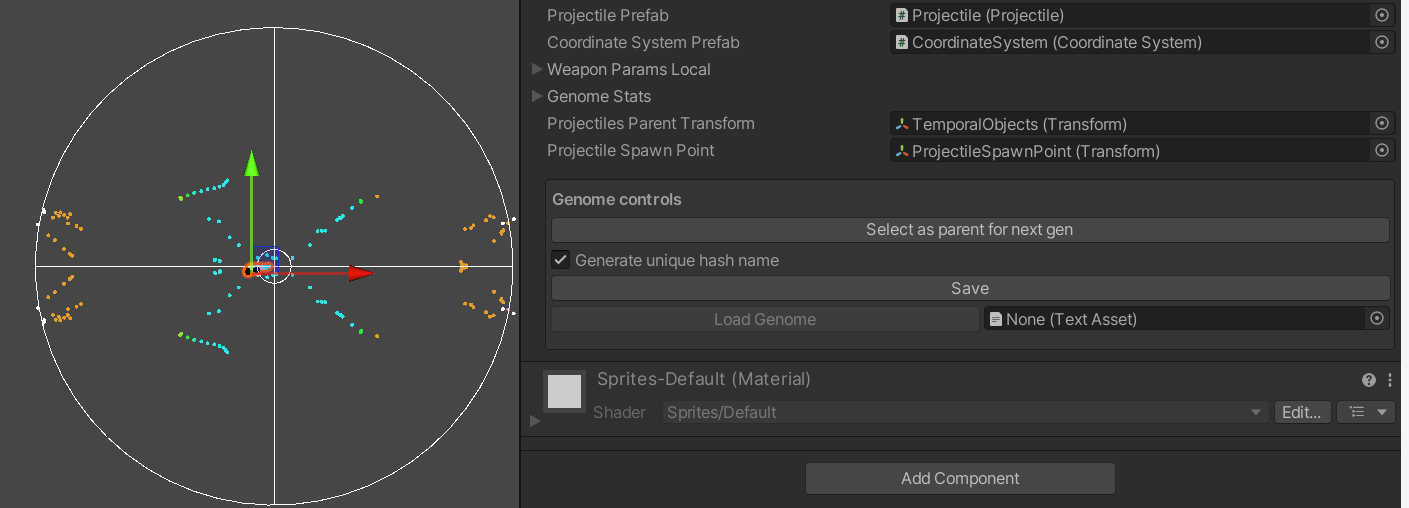
\includegraphics{images/SelectWeapon}
        }

        \caption{
            \label{SelectWeapon}
            Выбор родителей для нового поколения.}
    \end {center}
\end {figure}

Чтобы выбрать геном в качестве родителя, нужно выбрать игровой объект оружия и в его инспекторе нажать кнопку {\small \textbf{Select as parent for next gen}}. После того как нужное количество родителей было выбрано, нужно нажать на кнопку {\small \textbf{New Generation}}.

\begin{figure}[ht]
    \begin{center}
        \scalebox{0.24}{
            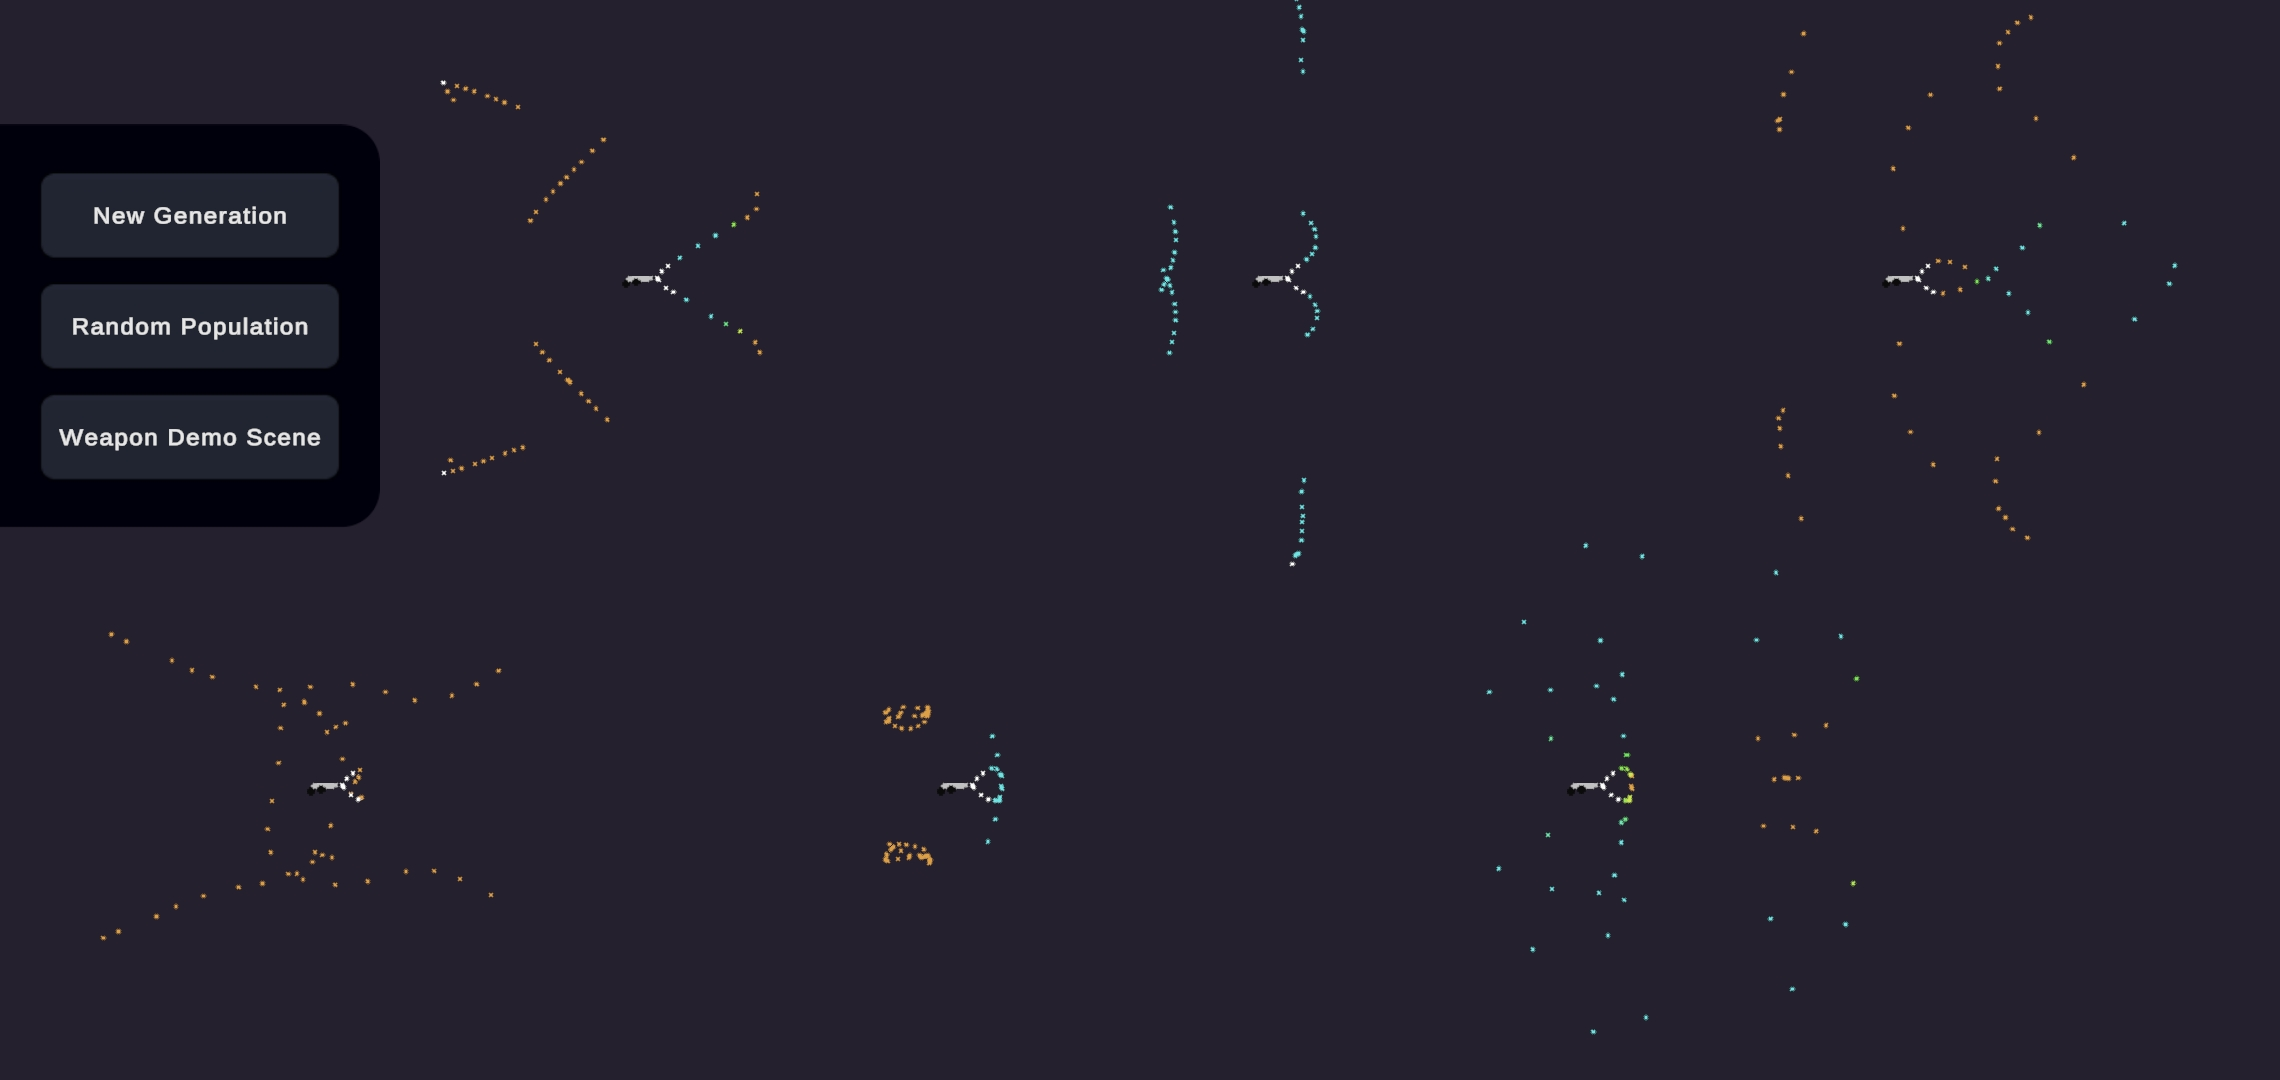
\includegraphics{images/EvoScene}
        }

        \caption{
            \label{EvoScene}
            Сцена эволюции оружия.}
    \end {center}
\end {figure}

Если эволюция зашла в тупик, нужно нажать на кнопку {\small \textbf{Random Population}}, которая создаст случайное поколение.

\subsection{Сохранение оружия}

Чтобы сохранить понравившееся оружие, нужно выбрать игровой объект оружия и в его инспекторе (Рисунок~\ref{SelectWeapon}) нажать кнопку {\small \textbf{Save.}} Будет создано и сохранено два файла:

\begin{enumerate}[label=\textbullet]
    \item {\small \textbf{Genome\_<UniqueHash>.xml}} содержит в себе информацию об узлах нейронной сети и функциях активации (Листинг~\ref{lst:xml}).
    \item {\small \textbf{Params\_<UniqueHash>.json}} является представлением параметров оружия в формате json (Листинг~\ref{lst:json}).
\end{enumerate}


\subsection{Сцена демонстрации оружия}

\textbf{Weapon Demo} -- сцена, в которой демонстрируется 140 оружий, подобранных разработчиком. В этой сцене есть визуализация силовых полей, действующих на снаряды. Силовое поле является визуализацией выводов нейронной сети:

\begin{enumerate}
    \item Направление стрелок передает значения выводов \textbf{x} и \textbf{y}.
    \item Размер стрелок передает значение вывода {\small \textbf{force}}.
    \item Цвет стрелок передает значение вывода {\small \textbf{hue}}.
\end{enumerate}

\begin{figure}[ht]
    \begin{center}
        \begin{minipage}[b]{0.38\textwidth}
            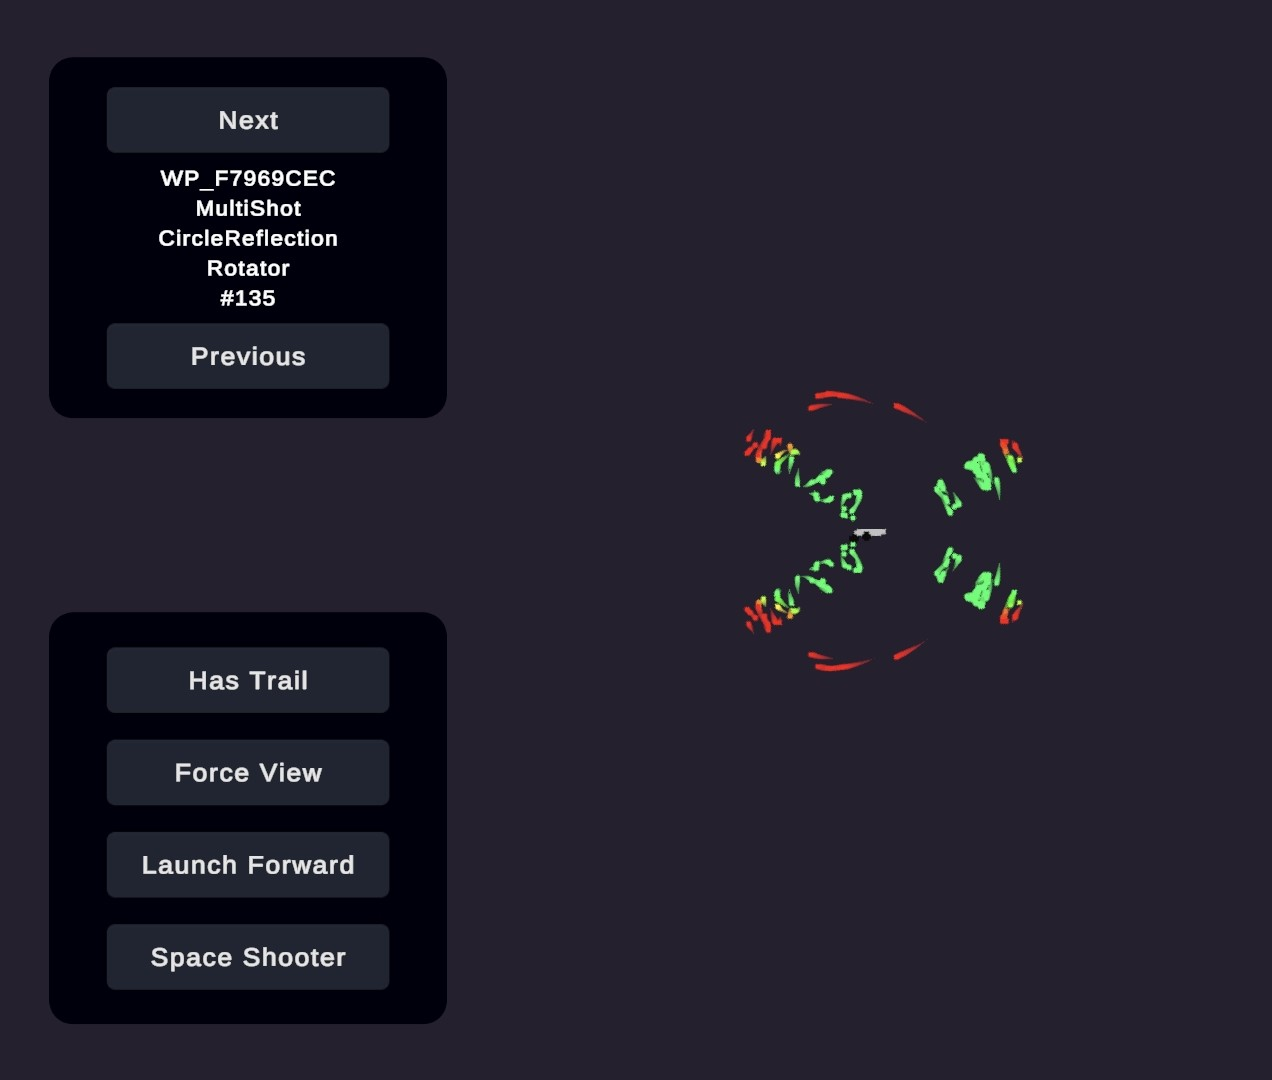
\includegraphics[width=\textwidth]{images/WeaponDemo1}
            \caption{
                \label{WeaponDemo1}
                Weapon Demo без визуализации силовых полей.}
        \end{minipage}
        \hspace{30pt}
        \begin{minipage}[b]{0.4\textwidth}
            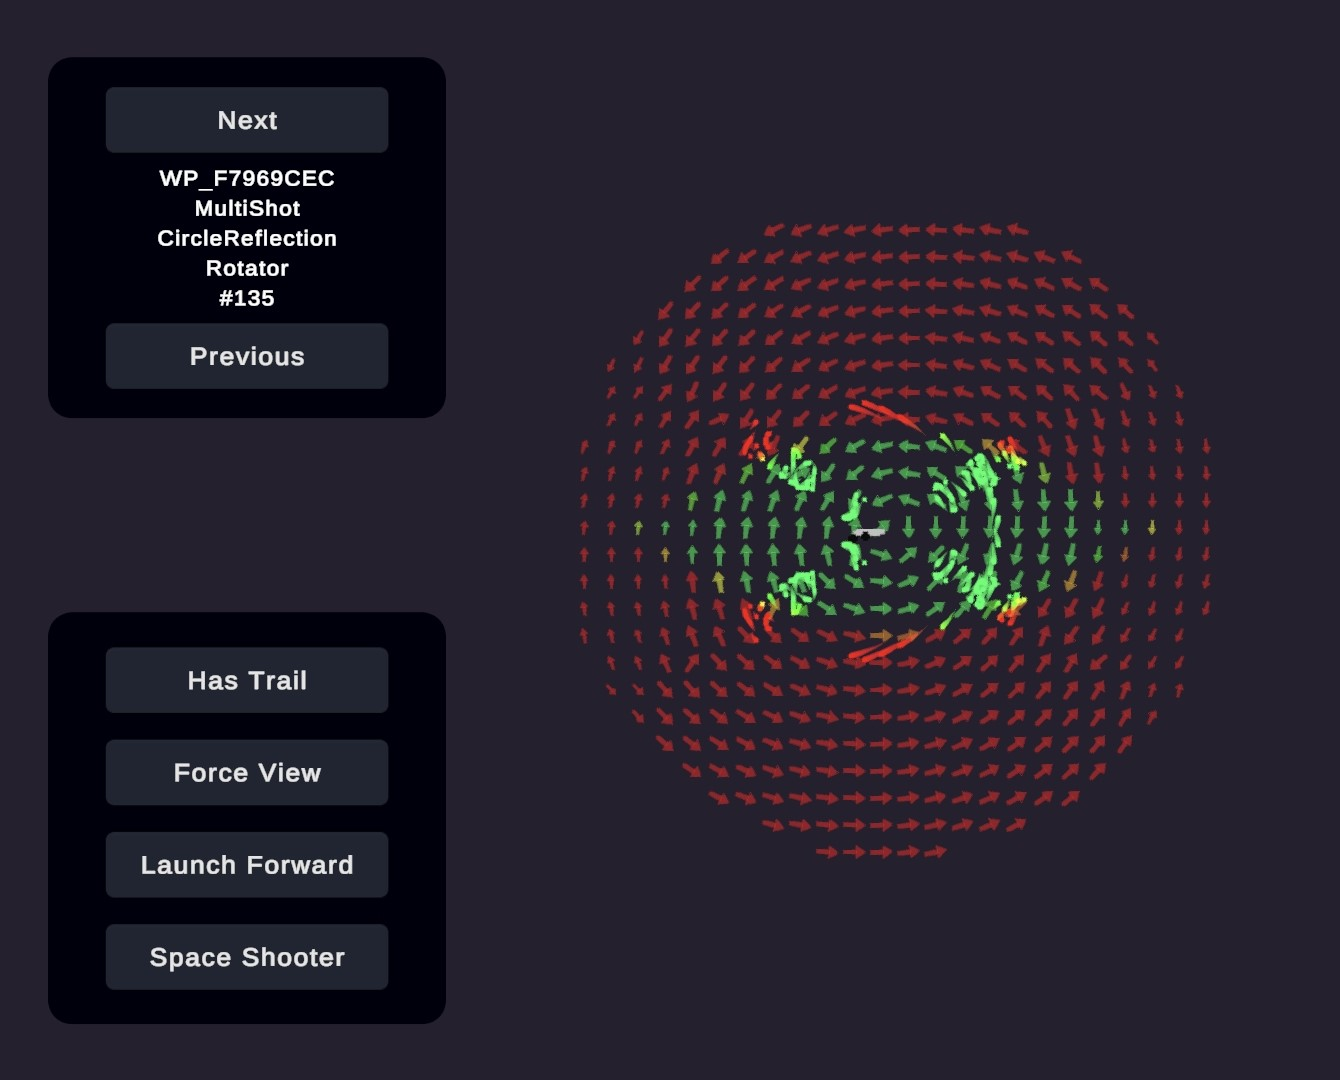
\includegraphics[width=\textwidth]{images/WeaponDemo2}
            \caption{
                \label{WeaponDemo2}
                Weapon Demo с визуализацией силовых полей.}
        \end{minipage}

    \end{center}
\end{figure}

\textbf{Замечание.} Разные группы снарядов имеют разные значения параметров {\small \textbf{SignY}} и {\small \textbf{SignX,}} иными словами, они по-разному интерпретируют выводы \textbf{x} и \textbf{y}, поэтому визуализация силового поля не может быть корректной для всех снарядов.\\
%
%
Функции этой сцены:
\begin{enumerate}[label=\textbullet]
    \item Кнопки {\small \textbf{Previous}} и {\small \textbf{Next}} для переключения оружия.
    \item В левом верхнем блоке интерфейса содержится информация о режимах оружия и его номер.
    \item Кнопка {\small \textbf{Has Trail}} определяет, оставляют ли снаряды за собой след.
    \item Кнопка {\small \textbf{Force View}} включает и выключает режим визуализации силовых полей.
    \item Кнопка {\small \textbf{Launch Forward}} запускает вперед системы координат, содержащие снаряды.
\end{enumerate}

